%-----------------------------------------------------------------------------%
\chapter{ANALISIS DAN PERANCANGAN SISTEM}

%-----------------------------------------------------------------------------%

%
\vspace{4.5pt}

Bab ini akan membahas tentang proses bisnis dan arsitektur dari rumah sakit Apertura. Lalu akan membahas analisa terkait proses bisnis dan arsitektur yang baru untuk diterapkan pada aplikasi, termasuk segala komponen penyusun sistem yang baru mulai dari database, \textit{tools}, IDE (\textit{Integrated Development Environment}), \textit{framework} yang digunakan dalam membangun aplikasi. Selanjutnya akan dibahas mengenai perancangan \textit{service} dengan menggunakan konsep REST dan pembuatan API dari \textit{service} tersebut.
\section{Arsitektur Monolitik pada Software Apertura}
Menurut Sam Newman, terdapat 2 parameter yang membedakan arsitektur monolitik dengan microservice, pertama adalah tingkat \textit{coupling} dan yang kedua adalah tingkat \textit{cohesion} dari aplikasi tersebut. Pernyataan ini kemudian didukung oleh Chris Richardson yang menjelaskan bahwa kedua parameter ini dapat ditinjau dari berbagai sisi yang membentuk aplikasi tersebut, antara lain: data menejemen, cara berkomunikasi, dan metode \textit{deployment} sebuah aplikasi.

\begin{enumerate}[leftmargin=*]
	\item \textbf{Data manajemen.} Aplikasi Apertura menerapkan model tersentralisasi yang sangat besar. Kurang lebih terdapat 120 tabel yang terdapat dalam 1 buah database tunggal. Namun semakin banyak model shared database yang digunakan, maka semakin tinggi pula derajat \textit{coupling} aplikasi tersebut, dan tingginya derajat \textit{coupling} merupakan salah satu ciri dari monolitik.
	\item \textbf{Cara berkomunikasi.} Modul dalam database Apertura dapat mengakses langsung tabel milik modul lain dengan melakukan \textit{querry} terhadap tabel tersebut. Cara berkomunikasi seperti ini seperti ini menjadi ciri dari arsitektur monolitik.
	\item \textbf{Bentuk deployment.} Tabel-tabel dan database Apertura disimpan dalam 1 buah database server yang sama. Penempatan server terpusat ini dianggap kurang menunjang konsep \textit{high availability} apabila terjadi masalah pada server. Aplikasi menjadi sangat tergantung dengan server tunggal tersebut dan menjadi ciri derajat \textit{coupling} yang tinggi.
\end{enumerate}
\newpage
Berdasarkan analisis dari ketiga faktor diatas, maka dapat disimpulkan bahwa arsitektur dari aplikasi Apertura adalah monolitik.\\
Arsitektur monolitik Apertura dapat digambarkan dengan deployment diagram dibawah:

\begin{adjustbox}{width=1\textwidth}
\begin{minipage}{\linewidth}
	\framebox[\textwidth]{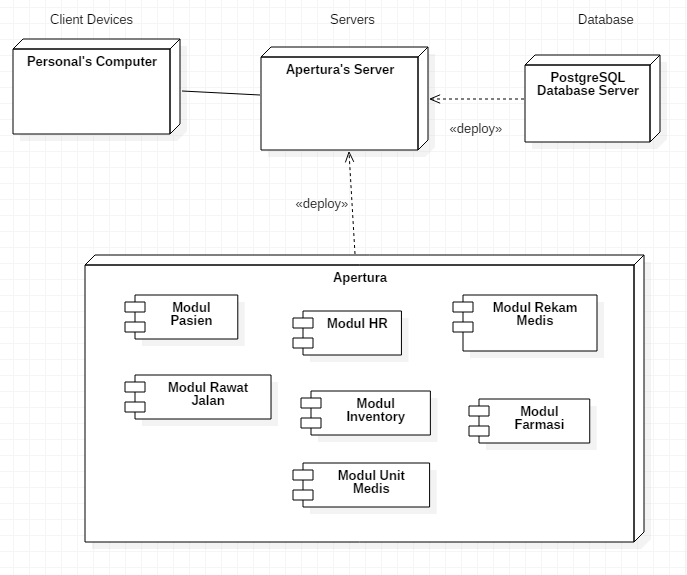
\includegraphics[width=10cm]{images/deployment_diagram.png}}	
	\captionof{figure}{Pemodelan Software Apertura dengan deployment diagram.}
\end{minipage}
\end{adjustbox}

\section{Tinjauan Umum Proses Bisnis Pelayanan Rawat Jalan}
Proses bisnis dalam rumah sakit Apertura melibatkan beberapa modul yang saling berinteraksi, modul-modul tersebut terdiri dari bagian yang lebih kecil lagi. Analisis berdasarkan proses bisnis berdasarkan kegunaannya akan lebih mudah untuk menentukan service yang akan terbentuk nantinya.\\
Modul-modul dari aplikasi Apertura antara lain: modul pasien, modul HR (human resources) yang meliputi data dokter, bidan, dan perawat, modul rekam medis, modul farmasi, modul inventori, modul akunting dan finansial, modul invoicing  dan pembayaran, modul rawat jalan, modul rawat inap, modul pemeriksaan penunjang, dan modul integrasi SEP (Surat Eligibilitas Pasien) BPJS.

Dari semua modul tersebut, penulis akan mengambil contoh kasus rawat jalan. Rawat jalan adalah tindakan perawatan pasien yang tidak menginap. Pasien yang datang akan mendaftar ke unit rawat jalan dan dicek apakah pasien tersebut terdaftar di BPJS, kemudian berdasarkan masalah pasien, pasien akan dirujuk ke unit medis yang ada di rumah sakit. Unit medis dari rumah sakit terdiri dari unit medis spesialis anak, spesialis jantung, dan spesialis penyakit dalam. Tiap unit medis memiliki satu atau lebih dokter spesialis dari bidang unit medis tersebut. Pasien kemudian akan ditangani oleh dokter yang bertugas di unit medis tersebut. Proses penanganan pasien dimulai dari konsultasi keluhan, pemeriksaan penunjang, dan diagnosis penyakit.

Hasil dari pemeriksaan tersebut akan disimpan dalam rekam medis pasien di rumah sakit. Modul rawat jalan akan mengeluarkan resep obat yang dapat pasien ambil di farmasi. Modul rawat jalan juga akan mengeluarkan detail faktur yang dibutuhkan untuk proses pembayaran. 

Maka dari itu, modul rawat jalan akan melibatkan modul pasien, HR, unit medis, farmasi, rekam medis, pemeriksa penunjang, pembayaran dan penagihan, integrasi BPJS, dan modul rawat jalan itu sendiri.\\
Berikut adalah penggambaran proses bisnis dari pelayanan rawat jalan:

\begin{adjustbox}{width=1\textwidth}
	\begin{minipage}{\linewidth}
		\framebox[\textwidth]{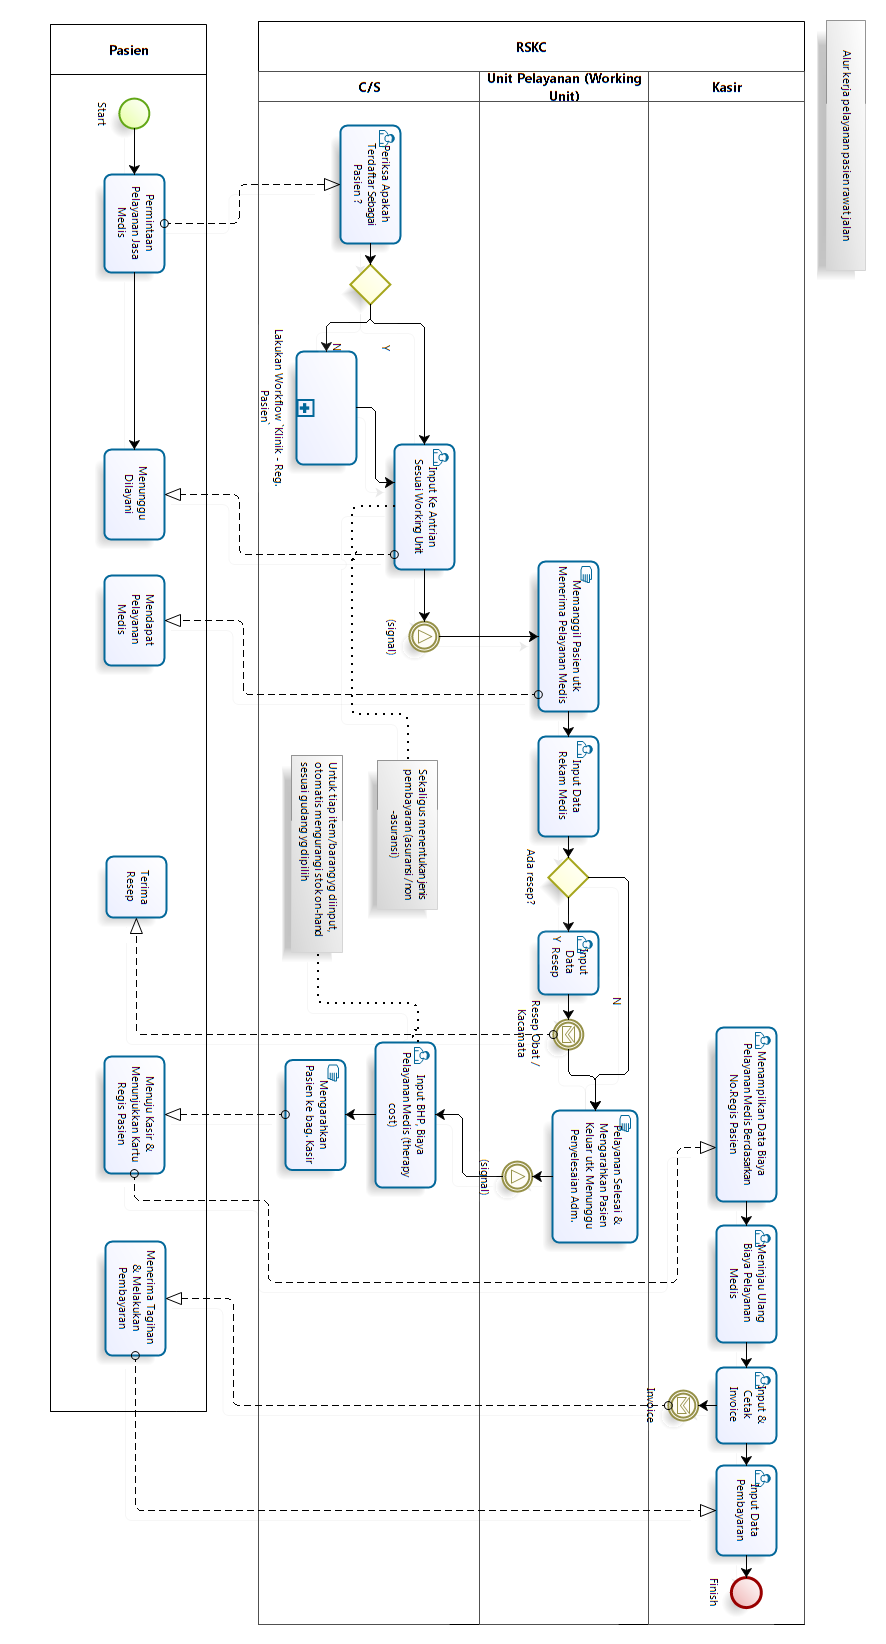
\includegraphics[width=12cm]{images/workflow_proccess.png}}	
		\captionof{figure}{Proses bisnis rawat jalan.}
	\end{minipage}
\end{adjustbox}

\section{Pembahasan Modul dan Kelas Penyusun}
Pada bagian ini akan dijelaskan fungsi dan kelas-kelas dari setiap modul dalam kaitannya dengan proses bisnis di rumah sakit.

\begin{enumerate}[leftmargin=*]
	\item \textbf{Modul Pasien.} Modul pasien berfungsi untuk menyimpan, memperbaharui, pencarian, dan menampilkan data pasien. Data pasien juga meliputi detail lengkap dari data keluarga atau kerabat yang menjadi penanggung jawab pasien. Kelas dari modul pasien adalah pasien itu sendiri.
	\item \textbf{Modul \textit{Human Resource}.} \textit{Human Resource} adalah modul yang mengelola semua pengguna dan pegawai dalam rumah sakit, modul ini dapat disebut juga sebagai modul karyawan. Beberapa contoh yang termasuk dalam modul ini adalah dokter, bidan, dan perawat. Modul ini menjadi modul dasar yang dibutuhkan modul lain, karena terkait pencatatan pengguna yang melakukan input data. Kelas-kelas dari modul ini meliputi dokter, bidan, dan perawat. Namun dalam contoh kasus rawat jalan yang akan diangkat, kelas yang diambil hanya dokter saja.
	\item \textbf{Modul Unit Medis.} Unit medis dari rumah sakit terdiri dari unit medis spesialis anak, spesialis jantung, dan spesialis penyakit dalam. Tiap unit medis memiliki satu atau lebih dokter spesialis dari bidang unit medis tersebut. Pasien akan ditangani oleh dokter yang bertugas di unit medis tersebut.
	\item \textbf{Modul Rekam Medis.} Rekam medis bertugas mencatat semua riwayat medis milik pasien yang meliputi hasil diagnosa, resep dan obat yang pernah diberikan, alergi, penyakit kronis, riwayat tindakan atau perawatan medis, dan hasil pemeriksaan penunjang. Pemeriksaan penunjang dapat berupa banyak aksi, tergantung apa yang dibutuhkan dokter. Pemeriksaan penunjang antara lain seperti radiologi, tes darah, tensi tekanan, dan lain lain. Fungsi dari pemeriksaan penunjang adalah menunjang ditegakannya diagnosis.
	\item \textbf{Modul Farmasi.} Modul farmasi bertugas untuk mengatur dan menyimpan obat-obatan. Modul farmasi menerima permintaan obat dari bagian IGD, rawat inap, rawat jalan, dan juga penjualan umum. Dalam aplikasi Apertura, modul ini juga meliputi fungsi dari apotek. Untuk IGD, rawat inap, dan rawat jalan pasti akan memiliki resep, namun untuk penjualan obat umum dapat menggunakan resep rujukan maupun tidak.
	\item \textbf{Modul Inventori.} Inventori dibagi menjadi 2 tipe, yaitu barang dan jasa. Barang meliputi obat, alat kesehatan (alkes), dan barang selain obat dan alkes. Adapun jasa yang dimaksud adalah jasa pelayanan kesehatan yang disediakan rumah sakit. Inventori berkaitan langsung dengan modul farmasi, karena modul farmasi membutuhkan data barang yang dijual.
	\item \textbf{Modul Rawat Jalan.} Rawat jalan adalah pelayanan medis kepada pasien untuk tujuan perawatan tanpa mengharuskan pasien tersebut untuk menginap. Rawat jalan menjadi perantara interaksi dari pasien dengan unit medis, rawat jalan menyimpan data perawatan yang kemudian akan disimpan dalam rekam medis. Hasil dari rawat jalan akan kemudian dibutuhkan oleh bagian pembayaran dan juga farmasi.
\end{enumerate}

Berikut adalah penggambaran relasi dari modul rawat jalan menggunakan komponen diagram:

\begin{adjustbox}{width=1\textwidth}
	\begin{minipage}{\linewidth}
		\framebox[\textwidth]{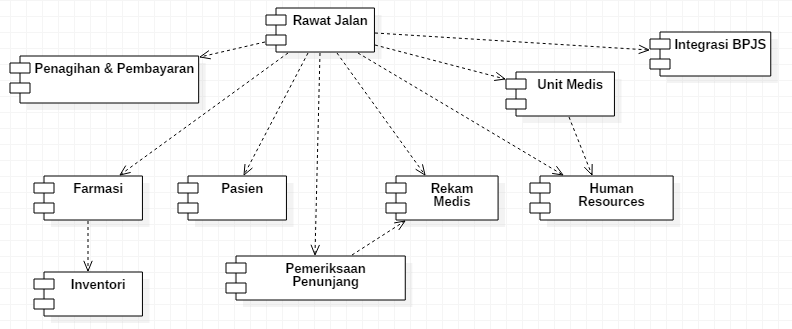
\includegraphics[width=13cm]{images/komponen_diagram_rawatjalan.png}}	
		\captionof{figure}{Komponen diagram rawat jalan.}
	\end{minipage}
\end{adjustbox}

\section{Identifikasi Teknologi yang Digunakan pada Aplikasi Apertura}
Saat ini teknologi aplikasi yang digunakan Rumah Sakit Apertura menggunakan arsitektur monolitik dengan database yang tersentralisasi pada 1 buah server. Database Apertura sendiri menggunakan PostgreSQL 9. PostgreSQL merupakan salah satu object-relational database management system (ORDMS) yang tersedia secara \textit{open source}. Database Apertura terdiri dari kurang lebih 120 tabel yang saling berelasi. Aplikasi Apertura digunakan oleh beberapa kelompok pengguna, antara lain bagian kasir rumah sakit, registrasi rawat jalan, registrasi rawat inap, kasir apotik, kasir rawat jalan, dokter, staf administrasi umum, staf keuangan, staf rekam medis, staf administrasi BPJS.
Aplikasi Apertura diimplemetasikan untuk diakses dalam bentuk aplikasi desktop. \textit{User interface} yang ditampilkan dalam aplikasi tidak terpisah secara moduler, melainkan satu kesatuan aplikasi besar yang kemudian dipisahkan berdasarkan kebutuhan user yang menggunakan aplikasi.

\subsection{Kekurangan Arsitektur Monolitik}
Kelemahan dari sistem Apertura sebenarnya berkaitan dengan kelemahan dari arsitektur monolitik itu sendiri. Berdasarkan analisis yang dilakukan, kelemahan dari arsitektur monolitik itu sendiri adalah:

\begin{enumerate}[leftmargin=*]
	\item Tingkat \textit{coupling} yang terlalu tinggi. Semua modul dalam sistem saling terikat, mengakibatkan kendala dalam proses pengembangan sistem. Perubahan dalam 1 buah objek harus diketahui oleh objek lain. Proses \textit{deployment} akan terhambat karena apabila hendak melakukan tes terhadap 1 buah modul, maka keseluruhan aplikasi harus di jalankan, mengakibatkan beban hardware lebih besar dan memakan waktu lebih banyak.
	\item Penyimpanan data yang terpusat pada 1 buah tempat (database) kurang baik. Apabila database mengalami \textit{down}, maka keseluruhan modul dari aplikasi tidak bisa melakukan pekerjaannya.
	\item Isu keamanan. Penyimpanan data dalam 1 buah database tidak cukup aman. Misalnya ada pihak yang tidak berwenang berhasil mengakses database, maka seluruh data aplikasi akan bocor.
	\item Sistem tidak cukup baik ketika menangani banyak user. Sistem akan kewalahan apabila banyak pengguna yang melakukan request dalam satu waktu, isu yang ditimbulkan adalah performa.
\end{enumerate}

\section{Perancangan Arsitektur Microservice}
Dengan menggunakan pattern dekomposisi berdasarkan kemampuan bisnisnya, maka service yang akan terbentuk dapat dibayangkan berdasarkan modul bisnis itu sendiri. Dalam kasus rawat jalan yang diangkat, maka modul yang saling berelasi adalah modul \textit{customer}, modul HR, modul inventori, modul farmasi, dan modul rawat jalan. Ke 5 modul ini akan dibuat menjadi service yang mandiri.

\begin{adjustbox}{width=1\textwidth}
	\begin{minipage}{\linewidth}
		\framebox[\textwidth]{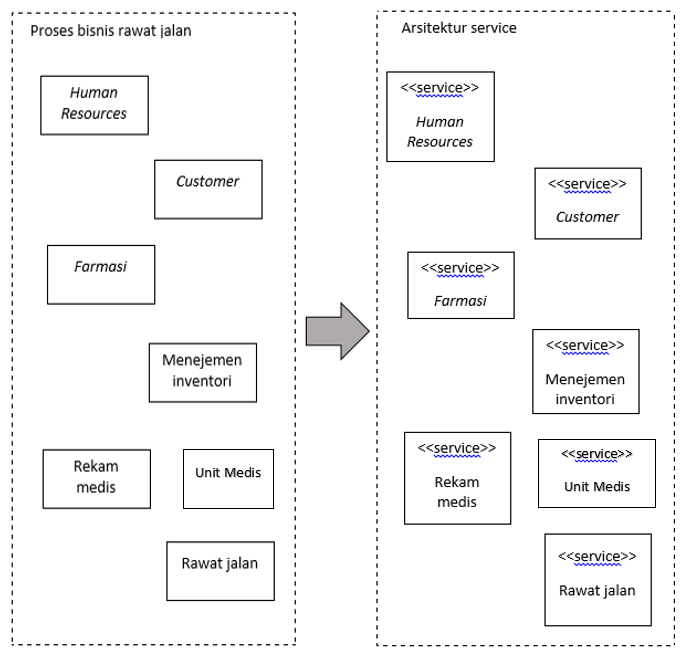
\includegraphics[width=12cm]{images/perancangan_modul.png}}	
		\captionof{figure}{Pembentukan service berdasarkan proses bisnis rawat jalan.}
	\end{minipage}
\end{adjustbox}

\subsection{Pemilihan Model Penyimpanan Data}
Setelah kelas-kelas service terbentuk, hal berikutnya yang harus diperhatikan adalah pemodelan manajemen data. Apabila ditinjau dari service yang dihasilkan, maka akan lebih baik menerapkan pattern database per \textit{service}, dimana satu service memiliki sebuah set database yang hanya bisa diakses oleh service tersebut dan tidak bisa saling mengakses database service yang lain.\\
Pemodelan database juga bergantung dengan bagaimana model database itu sendiri. Apabila model database yang digunakan nanti adalah \textit{relational database}, maka \textit{service} tersebut akan memiliki sebuah set database yang terdiri dari beberapa schema berhubungan yang hanya bisa diakses oleh \textit{service} tersebut. Apabila database yang digunakan adalah \textit{non-relational database}, maka cukup sebuah \textit{schema} tabel untuk 1 \textit{service}.
\subsection{Pemilihan Server Basisdata}
Aplikasi akan menggunakan 2 buah database untuk kegunaan yang berbeda. Database server yang pertama akan tetap sama seperti yang saat ini sistem gunakan yaitu PostgreSQL versi 9.4. Namun untuk kasus seperti rekam medis yang berbentuk multimedia (video, audio, foto) peneliti akan menggunakan MongoDB yang dinilai mudah, cepat, dan \textit{open source}. Walaupun database yang digunakan sama dengan yang digunakan oleh sistem sebelumnya, namun perancangan dalam database sangat berbeda terlebih setelah memilih model penyimpanan data.
\subsection{Pemilihan Komunikasi Antar Service}
Setelah membuat service dan database yang digunakan, hal berikutnya adalah membuat API dari service tersebut agar dapat diakses menggunakan \textit{web service}. Berdasarkan kebutuhan arsitektur microservice sendiri, model \textit{web service} yang akan digunakan adalah RESTful (\textit{Representational State Transfer}) dengan format data yang dikirim berupa JSON (\textit{JavaScript Object Notation}). Server sementara yang akan digunakan selama tahap perancangan adalah mesin pribadi milik peneliti. Setelah perancangan selesai dan siap, server baru akan dipindahkan ke server milik rumah sakit. Untuk tes pemanggilan API sementara dapat dilakukan dalam satu jaringan yang sama.
\subsection{Rancangan Deployment}
Model \textit{deployment} yang akan digunakan adalah \textit{multiple service per host}, dikarenakan lebih cocok dalam kasus penelitian yang hanya mengambill proses rawat jalan. Semua set service yang terbentuk akan di \textit{upload} dalam beberapa server agar dapat membuktikan tercapainya \textit{high availability}. Apertura sendiri memiliki 2 buah server aktif yang dapat digunakan ketika proses \textit{deployment}, serta server lainnya dapat menggunakan mesin pribadi untuk melakukan pemanggilan service dari server lain.

\section{Strategi Pengujian}
Strategi pengujian yang dirancang untuk kasus penulis adalah dengan melakukan uji perbandingan performa dengan arsitektur monolitik yang digunakan pada aplikasi saat ini. Tujuan dari test performa ini adalah menunjukan bahwa arsitektur microservice yang baru akan lebih unggul dalam 5 point diatas apabila dibandingkan dengan monolitik.
\subsection{Uji Perbandingan Performa}
Uji yang kedua adalah menunjukan bahwa performa dari arsitektur microservice akan memberikan hasil yang lebih baik dari monolitk. Strategi pengujian yang akan dilakukan adalah dengan membuat point-point pembanding yang akan diuji, kemudian dari point tersebut akan dibuat \textit{test-plan} masing-masing yang terdiri dari sekitar 1-3 buah \textit{test-plan}. \textit{Test result} kemudian akan disimpan dalam dokumen berupa \textit{matrix traceability}.\\
Menurut Paulo Merson (\textit{Software Architecture} di TCU; \textit{SOA/microservice trainer dan consultant}), point pembanding tersebut adalah [12]:

\begin{enumerate}[leftmargin=*]
	\item \textit{Deployability}. Lebih agile untuk untuk meluncurkan versi terbaru karena siklus \textit{build, test, build} yang lebih pendek. Tingkat fleksibilitas yang lebih tinggi untuk menggunakan layanan keamanan, replikasi, persistensi, dan konfigurasi pemantauan.
	\item \textit{Reliability}. Kesalahan dalam microservice hanya akan berpengaruh pada microservice itu sendiri dan konsumennya, sedangkan dalam model monolitik kesalahan layanan dapat merusak seluruh sistem monolitik.
	\item \textit{Availability}. Waktu \textit{downtime} yang dibutuhkan ketika ingin mengeluarkan versi terbaru dari microservice lebih sedikit dibandingkan monolitik.
	\item \textit{Scalability}. Setiap microservice dapat diskalakan secara terpisah menggunakan \textit{pool, cluster, grid}. Karakter menyebar membuat microservice lebih fleksibel dibandingkan dengan monolitik.
	\item \textit{Modifiability and Management}. Sifat fleksibel untuk menggunakan \textit{framework, libraries}, dan sumber data baru karena ditunjang sifat \textit{loose-coupled} yang dimiliki microservice, modular komponen hanya dapat diakses oleh \textit{contracts} (pihak yang berhak), dan sifat yang cenderung tidak mudah berubah menjadi \textit{software} besar yang sulit ditangani. Upaya pengembangan aplikasi juga dapat dibagi dalam tim yang lebih kecil dan bekerja lebih mandiri.
\end{enumerate}

Tujuan dari test performa ini adalah menunjukan bahwa arsitektur microservice yang baru akan lebih unggul dalam 5 point diatas apabila dibandingkan dengan monolitik.

\section{Batasan Implementasi}
Adapun batasan implementasi dalam pengembangan aplikasi yaitu:

\begin{enumerate}[leftmargin=*]
	\item Server cloud yang dapat digunakan ada sebanyak 2 buah milik Apertura. Keterbatasan sumber daya menjadi hambatan dalam menambah server baru.
	\item Dikarenakan \textit{deployment} service ada yang dilakukan di server lokal (mesin pribadi), maka untuk kasus tersebut pemanggilan API dibatasi dalam 1 jaringan yang sama. 
\end{enumerate}
\section{Lingkungan Implementasi}
Adapun spesifikasi mesin pribadi ketika melakukan proses implementasi adalah sebagai berikut:

\begin{enumerate}[leftmargin=*]
	\item Perangkat keras: 1 buah komputer sebagai server, 1 buah komputer sebagai client.
	\item Spesifikasi komputer: 64-bit prosesor dan sistem operasi.
	\item OS: Windows 10 Pro.
	\item Processor: Intel(R) Core i3-4150 CPU, 3.50GHz
	\item Memory: 8 GB RAM.
	\item Storage: 50 MB.
	\item Integrated Development Environment (IDE): Netbeans atau Eclipse neon 3.
	\item Java version: 1.8.0
	\item DB : PostgreSQL 9.6
\end{enumerate}